\documentclass[conference]{IEEEtran}
\IEEEoverridecommandlockouts
% The preceding line is only needed to identify funding in the first footnote. If that is unneeded, please comment it out.
\usepackage{cite}
\usepackage{amsmath,amssymb,amsfonts}
\usepackage{algorithmic}
\usepackage{graphicx}
\usepackage{textcomp}
\usepackage{xcolor}
\usepackage{dblfloatfix}
\def\BibTeX{{\rm B\kern-.05em{\sc i\kern-.025em b}\kern-.08em
    T\kern-.1667em\lower.7ex\hbox{E}\kern-.125emX}}
\begin{document}

\title{PointNet meets Self-Attention Graph Pooling: A Synergistic Approach to Point Cloud Classification 
\\
}

\author{
\IEEEauthorblockN{1\textsuperscript{st} M. Ebadpour}
\IEEEauthorblockA{\textit{Master of Science student} \\
\textit{Amirkabir university of technology}\\
Tehran, Iran \\
M.Ebadpour@aut.ac.ir}
\and
\IEEEauthorblockN{2\textsuperscript{nd} M. Javanmardi}
\IEEEauthorblockA{\textit{Assistant Professor} \\
\textit{Amirkabir university of technology}\\
Tehran, Iran \\
MJavan@aut.ac.ir}
\and
\IEEEauthorblockN{3\textsuperscript{rd} M. Choupan}
\IEEEauthorblockA{\textit{bachelor of science} \\
\textit{Amirkabir university of technology}\\
Tehran, Iran \\
Mohamadkhoee@aut.ac.ir}
\and
\IEEEauthorblockN{4\textsuperscript{th} M. Atyabi}
\IEEEauthorblockA{\textit{bachelor of science} \\
\textit{Amirkabir university of technology}\\
Tehran, Iran \\
atyabi2000@gmail.com}   

}

\maketitle

\begin{abstract}
% Point cloud is an important type of 3D data strucrue which has an important rule in researchs about our invoiroment
% and has wise application in industry such as autonomous driving, image segmentation and ... .
% On the other hand, graphs are usefull data structure to regulize point cloud data and we can add graph fetures to point cloud data 
% for extract some features for each point in data. graph based neural networks can help us to extract fetures from point cloud data in the way 
% each point specific features are conculed in classification result and this could improve detection accuracy.
% in this paper we explore the effect of graph centrality fetures on each point using Point-Net and Self-Attention Graph Polling as baselines and Also implement two new architecture for point cloud classification.
% The first architecture combines Poin-Net and Self-Attention Graph Pooling model using fusion approches. Second model is a Poin-Net based Self-Attention Graph Pooling which 
% use first model result as the second model input. Extensive experiments were conducted on the ModelNet10 dataset, results are showing Closeness and harmonic centralities are improve the 
% classification accuracy . as the total accuracy improve 3%
%  compared to the individual architectures, while also reducing model size 1MB. 

The point cloud is a crucial 3D data structure that plays a significant role in environmental research and has extensive 
applications in industries such as autonomous driving and image segmentation.
 Additionally, graphs are useful data structures for regularizing point cloud data,
  allowing the incorporation of graph features to extract specific attributes for each point 
  in the dataset. Graph-based neural networks facilitate the extraction of features from point
   cloud data, ensuring that each point's unique characteristics contribute to the classification 
   results, thereby enhancing detection accuracy.
In this paper, we investigate the impact of graph centrality features on each point using
 Point-Net and Self-Attention Graph Pooling as baselines. We also introduce two novel architectures 
 for point cloud classification. The first architecture integrates the Point-Net and Self-Attention Graph 
 Pooling models using fusion approaches. The second model is a Point-Net based Self-Attention Graph Pooling,
  which utilizes the results from the first model as input for the second. Extensive experiments conducted on
   the ModelNet10 dataset demonstrate that the inclusion of Closeness and Harmonic centralities are the bset centralies for classification.
   our new architectures improves classification accuracy by 4.7\% compared to the individual architectures, while also reducing the model size by 1MB.


\end{abstract}

\begin{IEEEkeywords}
Point Cloud Classification, PointNet, Self-Attention Graph Pooling, 3D Object Recognition.
\end{IEEEkeywords}

\section{Introduction}
{
    \color{red}
    [skipped]
}
\section{Related Works}
{
    \color{red}
    [should be done by Ms.Atybai]
}

\section{PROPOSED APPROACHES}
\subsection{Feature Engineering }\label{AA}
In this section, we present our approach to feature engineering in point cloud classification due to the limitations of XYZ features.
 To enhance feature representation, we exploit graph-based features, starting with the construction of a weighted and directed graph
  using the k-nearest neighbors method. As we consider the inherent 3D spatial relationships, we set K to 6, representing the six absolute
   sides in 3D space. This graph enables efficient feature aggregation and captures crucial spatial dependencies among points.

To further enrich the feature set, we introduce node centrality as an essential feature for each node (point in space)
 within the graph. We employ seven centrality metrics, namely betweenness, closeness, Katz, PageRank, eigenvector, harmonic,
  and load centrality.
\begin{itemize}
    \item Betweenness: This centrality feature measures the importance of a node in connecting other nodes.
    Mathematically, let $n_{s,t}^{i}$ be the number of geodesic paths from $s$ to $t$ that pass through $i$ and 
    let $n_{s,t}$ be the total number of geodesic paths from $s$ to $t$. Recall that a geodesic path is not necessarily 
    unique and the geodesic paths between a pair of vertices need not be node-independent, meaning they may pass through 
    some of the same vertices. Then the betweenness centrality of vertex $i$ is calculated by equation \ref{eq:beetweennes}:
    \begin{equation}\label{eq:beetweennes}
        b_i = \sum_{s, t} w_{s,t}^{i} = \sum_{s, t} \frac{n_{s,t}^{i}}{n_{s,t}}
    \end{equation}
    \item Closeness: closeness centrality (or closeness) of a node is a measure of centrality in a network, 
    calculated as the sum of the length of the shortest paths between the node and all other nodes in the graph.
    Thus the more central a node is, the closer it is to all other nodes. The closeness centrality of node $x$ is calculated by equation \ref{eq:closeness}.
    where $d(y,x)$ is the distance between vertices $x$ and $y$.
    \begin{equation}\label{eq:closeness}
        C(x) = \frac{N}{\sum_{y}^{}d(y,x)}
    \end{equation}
    \item Katz: Katz centrality computes the relative influence of a node within a network by measuring
     the number of the immediate neighbors (first degree nodes) and also all other nodes in the network that connect
      to the node under consideration through these immediate neighbors. In summary it combines both local and global node information.
      For calculate Katz for a node Let $A = (a_{i,j})$ be the adjacency matrix of a directed graph. The Katz centrality $x_{i}$ of node $i$ is given by: $$x_i = \alpha \sum_k a_{k,i} \, x_k + \beta$$ where $\alpha$ and $\beta$ are constants. In matrix form we have: $$x = \alpha x A + \beta$$ where $\beta$ is now a vector whose elements are all equal a given positive constant. 
      The free parameter $\alpha$, known as the damping factor, should be chosen with case. For small (close to 0) values of $\alpha$ the contribution given by paths longer than one rapidly declines, and thus Katz scores are mainly influenced by short paths (mostly in-degrees) and by the exogenous factor of the system.
    \item PageRank: PageRank is an adjustment of Katz centrality that takes into consideration this issue. There are three distinct factors that determine the PageRank 
    of a node: (i) the number of links it receives, (ii) the link propensity of the linkers, and (iii) the centrality of the linkers. 
    The first factor is not surprising: the more links a node attracts, the more important it is perceived
    For calculate PageRank for a node Let $A = (a_{i,j})$ be the adjacency matrix of a directed graph. The PageRank centrality $x_{i}$ of node $i$ is given by: $$x_i = \alpha \sum_k \frac{a_{k,i}}{d_k} \, x_k + \beta$$ where $\alpha$ and $\beta$ are constants and $d_k$ is the out-degree of node $k$ if such degree is positive, or $d_k = 1$ if the out-degree of $k$ is null. In matrix form we have: $$x = \alpha x D^{-1}A + \beta$$ where $\beta$ is now a vector whose elements are all equal a given positive constant and $D^{-1}$ is a diagonal matrix with $i$-th diagonal element equal to $1/d_{i}$. Notice that, as seen for Katz centrality, PageRank is determined by an endogenous component that takes into consideration the network topology and by an exogenous component that is independent of the network structure. It follows that $x$ can be computed as: $$x = \beta (I - \alpha D^{-1}A)^{-1}$$

    The damping factor $\alpha$ and the personalization vector $\beta$ have the same role seen for Katz centrality.
     In particular, $\alpha$ should be chosen between $0$ and $1 / \rho(D^{-1}A)$. Also, when the network is large,
      it is preferable to use the power method for the computation of PageRank.
    \item Eigenvector: Eigenvector centrality (also called eigencentrality) is a measure of the influence of a node 
    in a network. It assigns relative scores to all nodes in the network based on the concept that connections to
     high-scoring nodes contribute more to the score of the node in question than equal connections to low-scoring nodes. 
     PageRank and the Katz centrality are variants of the eigenvector centrality. Using the adjacency matrix to find 
     eigenvector centrality For a given graph $G := (V,E)$ with $|V|$ verticces let $A = (a_{v,t})$ be the adjacency matrix, i.e.
     $a_{v,t} = 1$ if vertex $v$ is linked to vertex $t$, and $a_{v,t} = 0 $ other wise. The relative centrality score of vertex $v$ can be defined as:
     $$ x_{v} = \frac{1}{\lambda}\sum_{t\epsilon M(v)}, x_{t} =\frac{1}{\lambda} \sum_{t\epsilon G} a_{v,t}x_t $$
    \item Harmonic: Harmonic centrality measures the 'average' distance of a node to the other nodes in the network. 
    This can be used to find nodes in a network that can quickly communicate with other nodes.
    For calculation harmonic centrality for node i let $d_(i,x)$ is a distance from node i to node x for a given graph $G := (V,E)$ with $|V|$ verticces then :
    $$ Harmonic(i) = \sum_{x\epsilon G , x \neq i } \frac{1}{d_(i,x)}$$
    \item Load centrality: The load centrality of a node is the fraction of all shortest paths that pass through that node. It 
     measures the node's importance in graph connectivity and load distribution. For calculate load centrality  Consider a graph $G := (V,E)$ and an
     algorithm to identify the (potentially multiple) minimum weight
     path(s) between any pair of vertices $(s, d)$. Let $\theta_{s,d}$ be a quantity
     of a commodity that is sent from vertex $s$ to vertex $d$. We
     assume the commodity is always passed to the next hop following
     the minimum weight paths. In case of multiple next hops, the
     commodity is divided equally among them. We call $\theta_{(s,d)}(v)$ the
     amount of commodity forwarded by vertex $v$. The load centrality
     of $v$ is then given by:
     $$LC(v) = \sum_{s,d \epsilon V} \theta_{(s,d)}(v)$$
\end{itemize}
\begin{figure*}[!h]
    \centering
    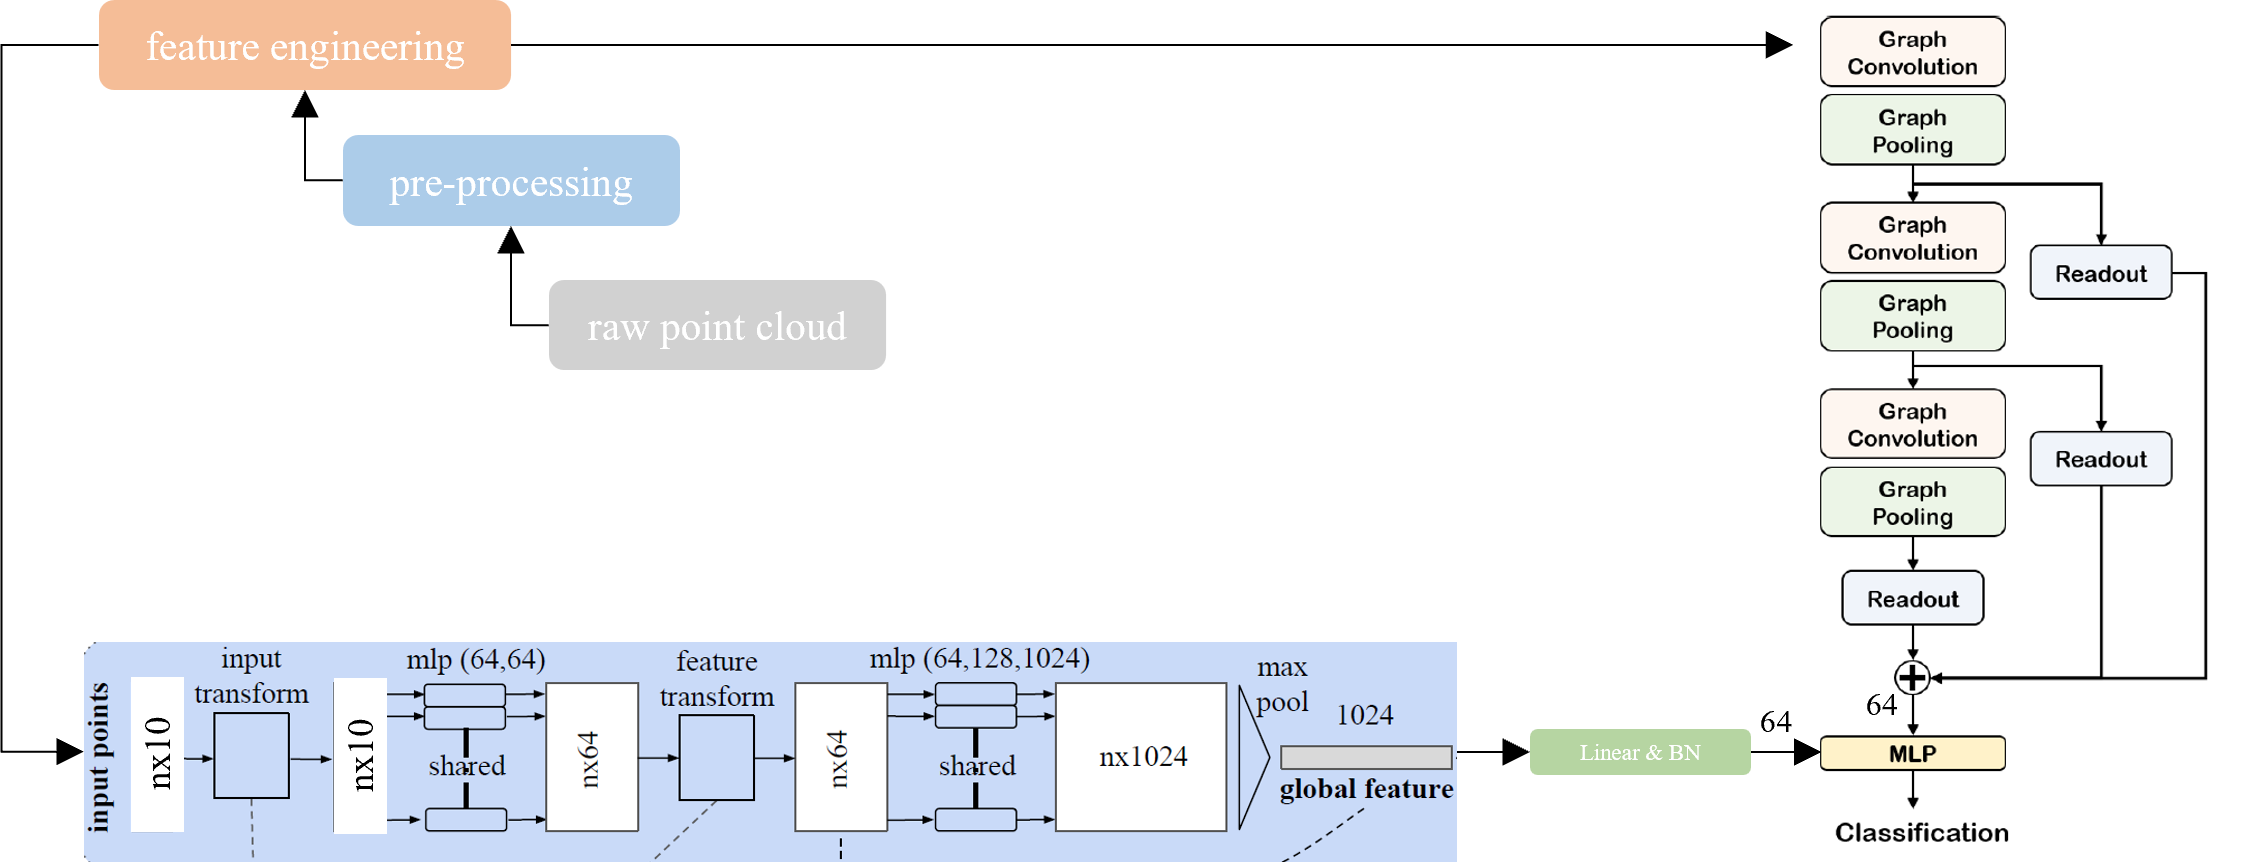
\includegraphics{fig1.png}
    \caption{The architecture for Feature Concatenation Approach.}
    \label{fig2}
\end{figure*}
%    Betweenness measures the importance of a node in connecting other nodes, while closeness evaluates how central a 
%   node is in terms of its average distance to all other nodes. Katz centrality combines both local and global node information,
%    and PageRank identifies nodes of significant influence. Eigenvector centrality evaluates the influence of a node based on the influence
%     of its neighbors. Harmonic and load centrality measure the node's importance in graph connectivity and load distribution, respectively.
% as the result shown in next section x,y are the best fetures which added to point cloud x,y,z and we used them for continue the approach
In our feature engineering process, we combine the seven centrality features with the existing XYZ features (x, y, and z coordinates)
 for each node. This results in a feature vector comprising 10 distinctive elements per point in the point cloud. Additionally,
  we applied a 1024 sampling rate to each point cloud to handle varying point densities efficiently. To ensure uniformity,
   we performed normalization across the feature vectors. Furthermore, random noise was introduced to augment the dataset,
    enhancing the model's robustness to real-world scenarios and improving generalization performance. These feature engineering 
    techniques aim to provide a comprehensive and informative representation of the point cloud data, optimizing the classification 
    performance in the subsequent stages of our research.
As shown in the subsequent section, the features closeness and harmonic are identified as the most effective additions to the point cloud's existing x, y, and 
z dimensions. These features were subsequently utilized to advance our approach.


It is important to note that the calculation of feature vectors for node centralities was implemented using multi-proccessing on the CPU.
 This approach allowed us to efficiently compute centrality metrics for each node in the point cloud concurrently, significantly reducing
  the computation time. By leveraging the power of multi-proccessing, we were able to accelerate the feature engineering process and 
  efficiently handle large datasets, ultimately improving the overall efficiency and performance of the fusion approaches.

% we choose Point-Net and Self-Attention Graph polling models as a baslines for improving. because Point-Net is a generel bechmark model for point cloud classification 
% and if we can achieve a better result in this base line it can be improved in other baseline . As the same for Self-Attention graph pooling is a popular benchmark
% in graph classification and better result generalization on other baselinse

We selected Point-Net and Self-Attention Graph Pooling models as baselines for improvement. 
Point-Net is a general benchmark model for point cloud classification, suggesting that any enhancements
 achieved with this baseline could potentially be replicated with other models. Similarly, Self-Attention 
 Graph Pooling is a popular benchmark in graph classification, and achieving better results with this model 
 could indicate improved generalization across other baselines.

\subsection{Feature Concatenation Approach}

In this proposed fusion approach, named "FeatureConcatModel," we combine the high-level features obtained from PointNet and SAGPool networks for efficient point cloud classification. Both networks take point clouds with 10 defined features as input. SAGPool outputs vectors with 64 features for each point cloud in a batch.

To adapt PointNet, we introduce a linear layer, reducing the 1024 features to 64 features for each point cloud. Subsequently, we concatenate the 64-feature vectors from both PointNet and SAGPool, creating a unified vector with 128 features. This concatenated feature vector captures both the local and global information, ensuring a comprehensive representation of the point cloud data.
To further process the concatenated features, we employ three multi-layer perceptron (MLP) networks. The first MLP contains 64 neurons, followed by a second MLP with 32 neurons, and finally a third MLP with 10 neurons corresponding to the number of classes. Batch normalization is applied to all three MLPs, enhancing the model's stability and accelerating convergence.

We employ dropout techniques with a probability of 0.3 in the second layer, reducing overfitting and improving generalization performance. Additionally, we incorporate the Graph Attention (GAT) layer from SAGPool with 6 attention heads, considering the 6 nearest neighbors for each point.



\begin{figure*}[t]
\centering{
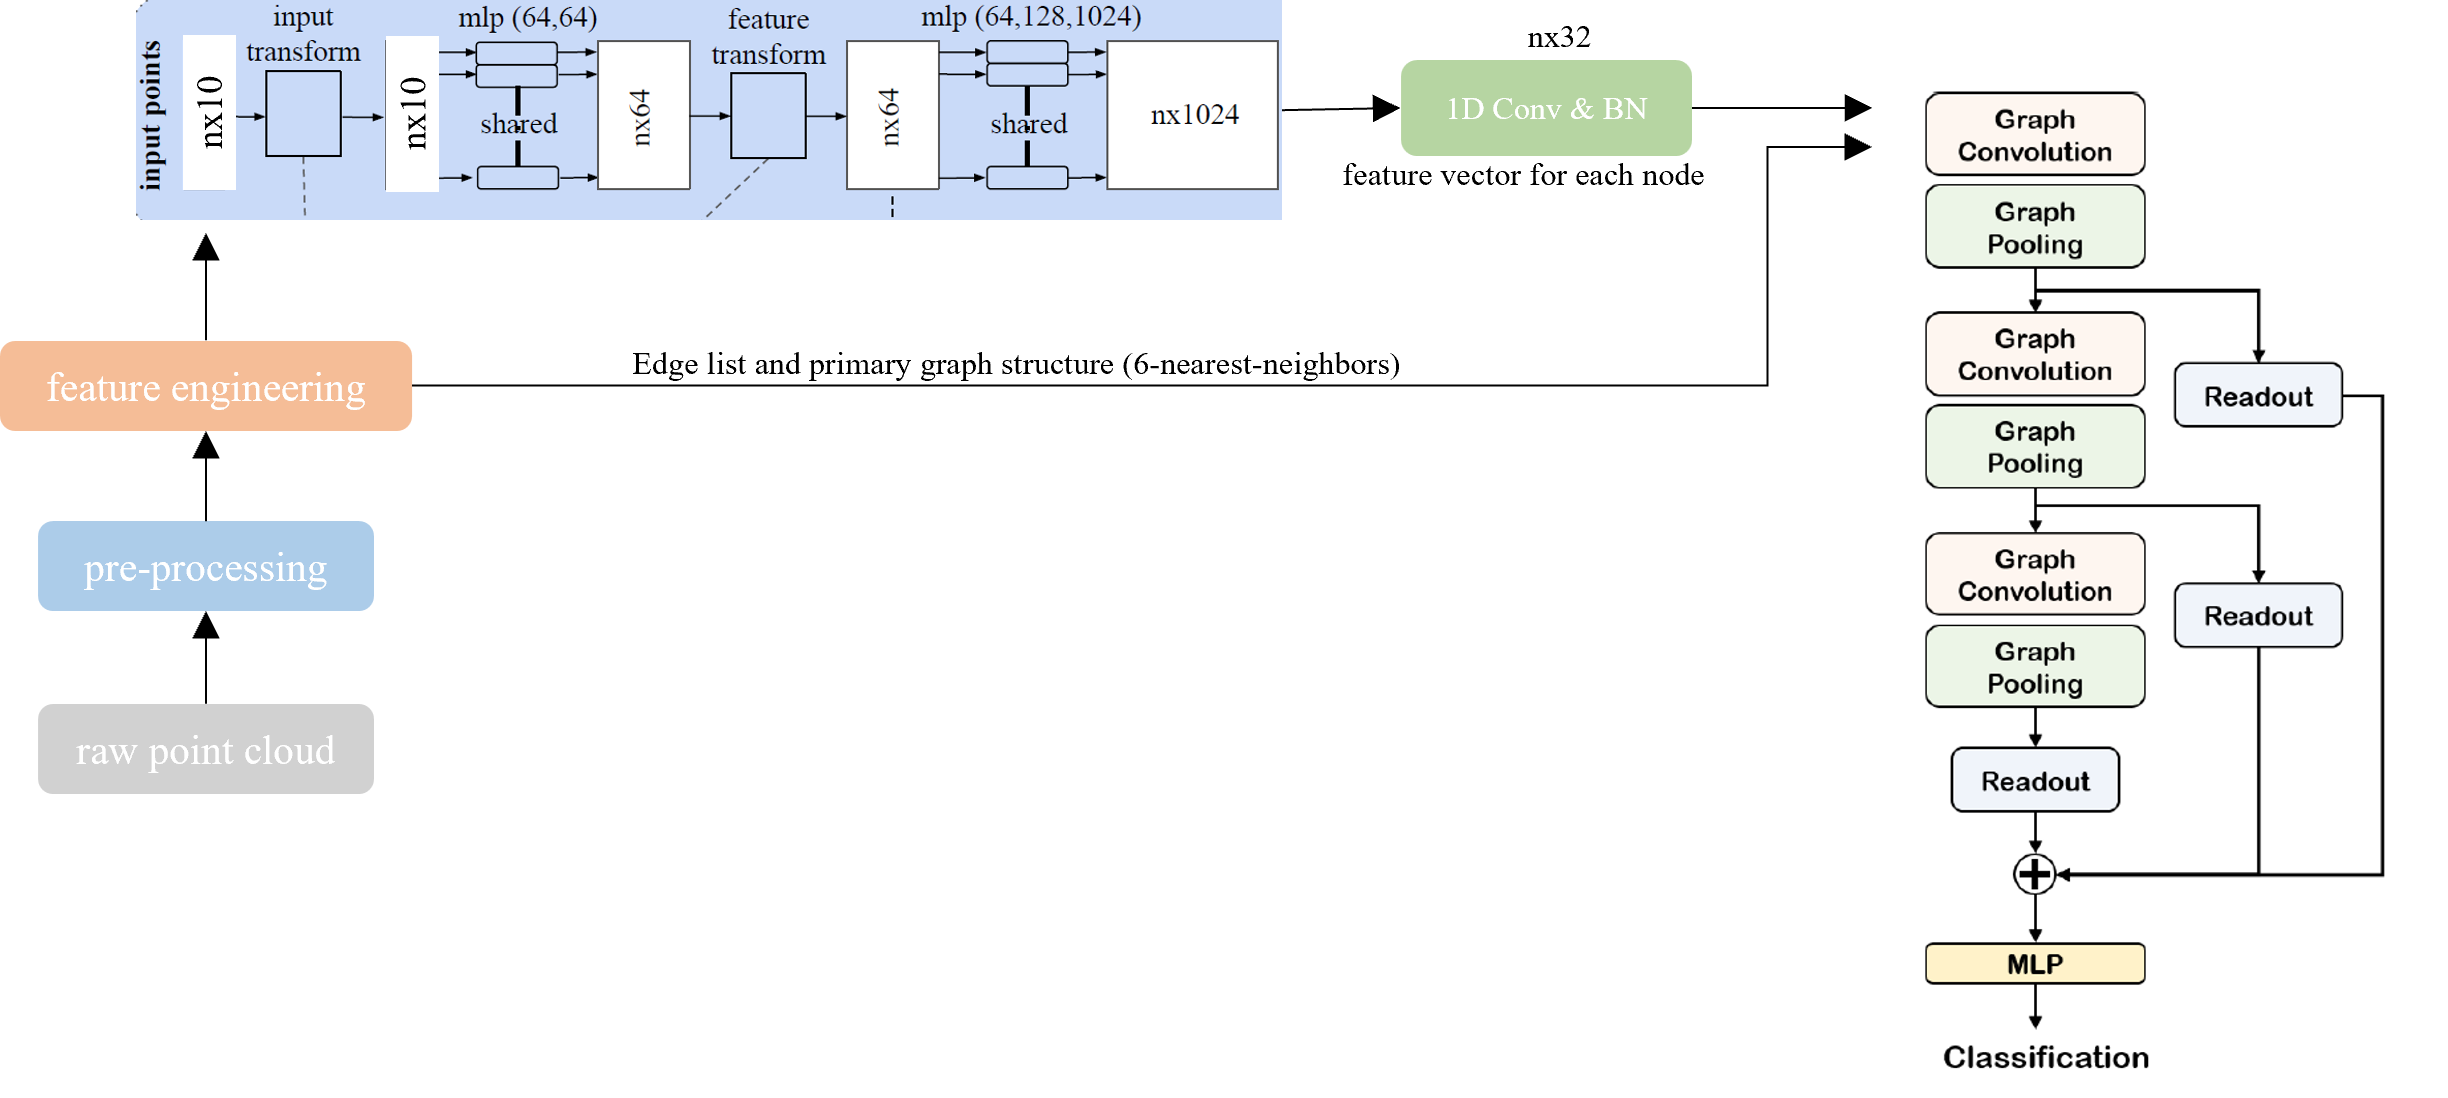
\includegraphics{fig2.png}}
\caption{The architecture for the graph classification based on PointNet features.}
\label{fig1}
\end{figure*}

This proposed "FeatureConcatModel" fusion approach offers a promising 
solution for point cloud classification, leveraging the strengths of both PointNet
 and SAGPool architectures. By effectively combining their high-level features,
  we aim to achieve improved classification accuracy and robustness in handling complex point cloud data.
   The architecture for feature concatenation is presented in ``Fig.~\ref{fig2}''. 


\subsection{Graph Classification based on PointNet Features}
The "PointNetBasedGraphPoolingModel" fusion approach represents a sophisticated integration of SAGPool and PointNet architectures,
 harnessing the strengths of both networks to enhance point cloud classification. To begin, we utilize a set of 10 defined features,
  including XYZ coordinates and centrality metrics, as input to the custom version of PointNet. In this custom implementation,
   we intentionally omit the global pooling section to obtain a 1024-feature vector for each node in the point cloud.
    This design choice enables PointNet to capture intricate local features and spatial relationships present in the data. 
    The architecture for the graph classification based on PointNet features is showcased in ``Fig.~\ref{fig1}''.


Subsequently, we enhance the feature vectors obtained from PointNet by applying 1D convolution, followed by batch normalization. This operation efficiently reduces the dimensionality to 32, effectively distilling essential information from PointNet's output. The resulting 32-feature vectors, carrying valuable local feature representations, are then fed into the SAGPool network.

SAGPool, with its primary edge list structure and consistent graph schema, efficiently performs adaptive feature pooling and aggregation. The integration of the PointNet-derived feature vectors into the SAGPool network further enhances its ability to capture meaningful global context while preserving crucial local details.

Experimental evaluations of the "PointNetBasedGraphPoolingModel" approach showcase its impressive performance in point cloud classification. By seamlessly blending the local feature extraction capabilities of PointNet with the adaptive feature aggregation of SAGPool, the approach achieves a more comprehensive representation of the point cloud data. The fusion of these two architectures leads to notable improvements in classification accuracy, enabling more robust, reducing the model size and accurate recognition of complex 3D scenes and objects.

The effectiveness of this fusion approach contributes significantly to the advancement of 3D perception and scene understanding applications. With its ability to leverage both global and local features, the "PointNetBasedGraphPoolingModel" approach exemplifies a powerful paradigm in point cloud classification and opens new avenues for future research and practical applications in various domains.


\section{EXPERIMENTS AND RESULTS}
\begin{figure*}[t!]
    \centering
    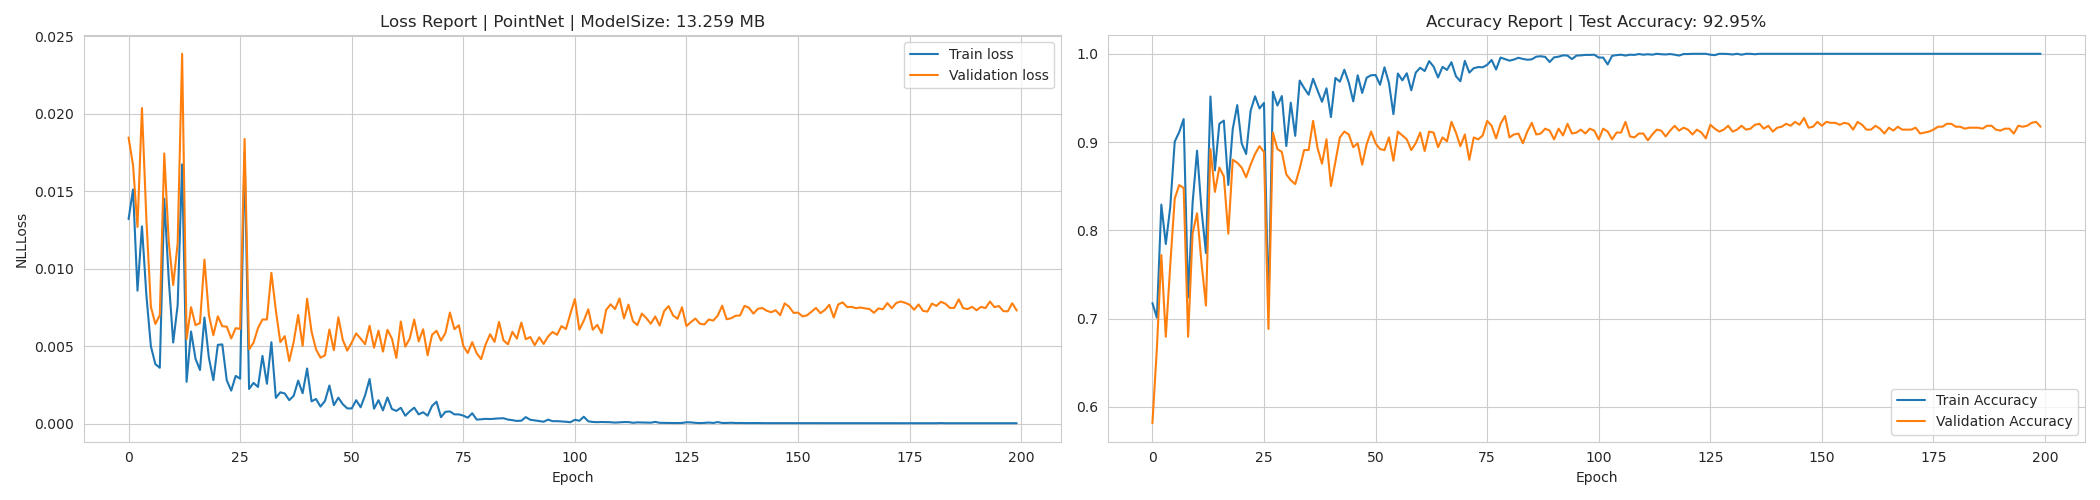
\includegraphics[height=4cm]{fig3.png}
    \caption{Training result for traditional PointNet Network On model Net 10.}
    \label{fig3}
    \end{figure*}
\subsection{Implementation details and hyper-parameters}
In our implementation, we adopted the PyTorch framework as the primary tool for model development. To facilitate graph pooling and centrality calculations, we incorporated PyTorch Geometric and NetworkX libraries, respectively. A comprehensive dataloader was designed, encompassing all

essential details, including XYZ features, graph edge lists, centrality features, and labels.

To optimize processing costs and expedite training, we employed parallel computation to precalculate and store the required features in separate files. During training, we efficiently loaded the precomputed features from the drive, minimizing redundant calculations and streamlining the training process.

For training and testing, we set the batch size to 32 and 64, respectively. Across all networks, a graph pooling rate of 0.25 was consistently applied, along with a Graph Attention (GAT) convolution layer featuring 6 heads and 128 hidden features.

The ADAM optimizer was chosen for training, with weight decay 0.0005 and learning rates of 0.01, 0.001, and 0.005 for the SAGPool, PointNet, and fusion approaches, respectively. Due to resource limitations during the research, we trained the networks for 60-200 epochs, allowing us to explore a wide range of model performance within our constraints.

Our experiments were conducted on a Desktop PC with a robust hardware configuration. The machine featured an Intel Core i7 12700K CPU, operating at 4.9 GHz frequency, and 32GB DDR5 main memory. Additionally, an Nvidia  RTX 3090 GPU with 8GB memory was utilized for accelerated computations.

In summary, our implementation details and well-optimized
hyperparameters ensured efficient and effective exploration of the fusion approaches' performance. While resource constraints influenced certain aspects of our experiments, the chosen hardware configuration allowed us to achieve substantial 
 progress in understanding the potential benefits of combining SAGPool and PointNet architectures for point cloud classification tasks.\\


\subsection{Dataset}


% The dataset used for training and testing the networks in this study is ModelNets. ModelNets are a widely used benchmark datasets in the field of 3D object recognition and classification.
%  It coculed ModelNet10 and ModelNet40 which have 10 and 40 classes. The categories in these datasets include common objects such as chairs, tables, airplanes, and cars, among others.

The dataset utilized for training and testing the networks in this study is ModelNet, a widely used benchmark in the field of 3D object recognition and classification. ModelNet comprises ModelNet10 and ModelNet40, which feature 10 and 40 classes, respectively. These datasets include categories of common objects such as chairs, tables, airplanes, and cars, among others
\begin{figure*}[b]
\centerline{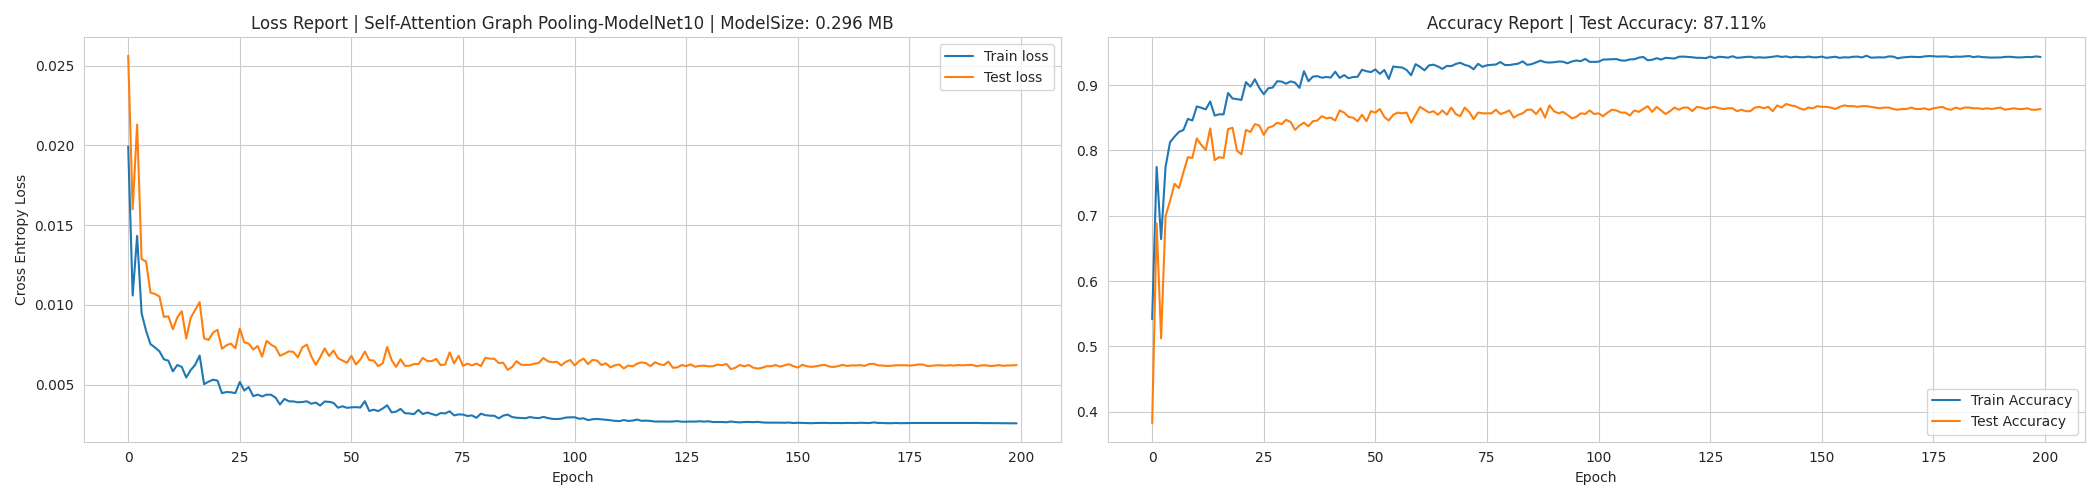
\includegraphics[width=\textwidth]{fig4.png}}
\caption{Training result for original hierarchical SAGPool network On model Net 10.}
\label{fig4}
\end{figure*}
To prepare the dataset for training and testing, several preprocessing steps were applied. Firstly, we employed a 1024 sampling rate to obtain a fixed number of points from each 3D model. This step ensured a consistent input size for the networks, facilitating efficient processing. Next, we applied normalization to scale the point coordinates, making them relative to the model's bounding box and ensuring that they lie within a common range. This normalization step enhanced the model's robustness and improved convergence during training.

Additionally, to augment the dataset and enhance the model's generalization capabilities, we introduced random noise to the point cloud data. This noise addition introduced small variations in the point positions, mimicking real-world scenarios and improving the network's ability to handle noisy input data. Furthermore, random rotation was applied to the 3D models during training. This augmentation technique involved rotating the objects along different axes, creating diverse orientations for each model. By doing so, the network learned to be invariant to object rotations, improving its ability to recognize and classify objects from different viewpoints.\\

To ensure an unbiased evaluation of the models' performance, the original ModelNet datasets
 was divided into predefined training and testing sets. The training set was used to train the fusion approaches, 
 while the testing set was kept separate for evaluation. This separation allowed for an objective assessment of the models'
  classification accuracy and generalization to unseen data. The utilization of the ModelNet10 dataset, combined with
   the various preprocessing and augmentation techniques, contributed to the robustness and effectiveness of the trained
    networks in point cloud classification tasks.


\subsection{Training }
In this section, we provide a detailed account of the training process for the four networks aimed at 
investigating the performance of the intersection of SAGPool and PointNet compared to each architecture used individually. 
For the first network, a traditional PointNet was trained using the standard ModelNet10 dataset with 3 features (XYZ coordinates). 
The results of this training are presented in ``Fig.~\ref{fig3}''.\\

The second network involved a hierarchical version of SAGPool with a custom improvement that incorporated 
learning weights for each stage. We trained this network using a feature vector of 10 dimensions, which included
 the XYZ coordinates along with centrality metrics. The training outcomes for this hierarchical SAGPool network 
 can be observed in ``Fig.~\ref{fig4}''.


Here's a revised version of your text:

Additionally, we examined the impact of each feature on the Point-Net and Self-Attention Graph Pooling baselines, 
with results presented in ``Table~\ref{tab2}``'' and ``Table~\ref{tab3}``'' .


These results demonstrate that Harmonic centrality is the most effective
 feature in the Self-Attention Graph Pooling model for both ModelNet10 and ModelNet40 datasets. This is because Harmonic
  centrality enhances the importance of points located on the edges of the point cloud data, which, followed by other features,
   yields the second-best result in this mode.

Conversely, in the Point-Net model, Katz centrality emerges as the best feature added to the base feature set.
 This is attributed to the model's T-net and feature extraction layer, which significantly influence shape recognition. 
 Katz Centrality specifically enhances feature extraction at the edges, similar to the Self-Attention Graph Pooling model.
  However, the primary difference between these two models lies in their architecture and their distinct approaches to impacting 
  the data.
  \begin{table}[t]
    
    \caption{Training Results of each feture on the Point-Net on ModelNet10 . The features used during training, test accuracy achieved are reported. The best-performing results are denoted by bold font, while the second-best results are italic, offering valuable insights into the performance of each feature}
    \begin{center}
    \begin{tabular}{|c|c|}
    \hline
      \textbf{\textit{Features}}& \textbf{\textit{Acc}} \\
    \hline
    3 (XYZ)&	\textit{91.85}\\
    \hline
    3 (XYZ) + Beetweennes&	92.29   \\
    \hline
    3 (XYZ)+ Closeness&	92.73  \\
    \hline
    3 (XYZ)+Eigenvector&	92.51 \\
    \hline
    3 (XYZ)+Harmonic&	92.29  \\
    \hline
    3 (XYZ)+Katz&\textbf{92.62}   \\
    \hline
    3 (XYZ)+Load centrality&	92.29   \\
    \hline
    3 (XYZ) + PageRank&	92.4   \\
    \hline
    All Features&	92.95   \\
    \hline

    \end{tabular}
    \label{tab2}
    
    \end{center}
    \end{table}
    
    \begin{table}[t]
    
        \caption{Training Results of each feture on the Self-Attention Graph pooling on ModelNet10 . The features used during training, test accuracy achieved are reported. The best-performing results are denoted by bold font, while the second-best results are italic, offering valuable insights into the performance of each feature}
        \begin{center}
        \begin{tabular}{|c|c|}
        \hline
          \textbf{\textit{Features}}& \textbf{\textit{Acc}} \\
        \hline
        3 (XYZ)&	87.11\\
        \hline
        3 (XYZ) + Beetweennes&	86.12   \\
        \hline
        3 (XYZ)+ Closeness&	83.26  \\
        \hline
        3 (XYZ)+Eigenvector&	87.33 \\
        \hline
        3 (XYZ)+Harmonic&	\textbf{87.89}  \\
        \hline
        3 (XYZ)+Katz&83.04   \\
        \hline
        3 (XYZ)+Load centrality&	87.56   \\
        \hline
        3 (XYZ) + PageRank&	87.22  \\
        \hline
        All Features&	\textit{87.78}   \\
        \hline
    
        \end{tabular}
        \label{tab3}
        
        \end{center}
        \end{table}
        

The third network implemented our proposed feature concatenation approach, where we combined the high-level features extracted from both PointNet and SAGPool networks.

Similarly, a feature vector of 10 dimensions, 
encompassing XYZ coordinates and centrality metrics,
 was used for training. The training results for this 
 feature concatenation approach are depicted in Fig.~\ref{fig7}''.
\begin{figure*}[t]
\centering{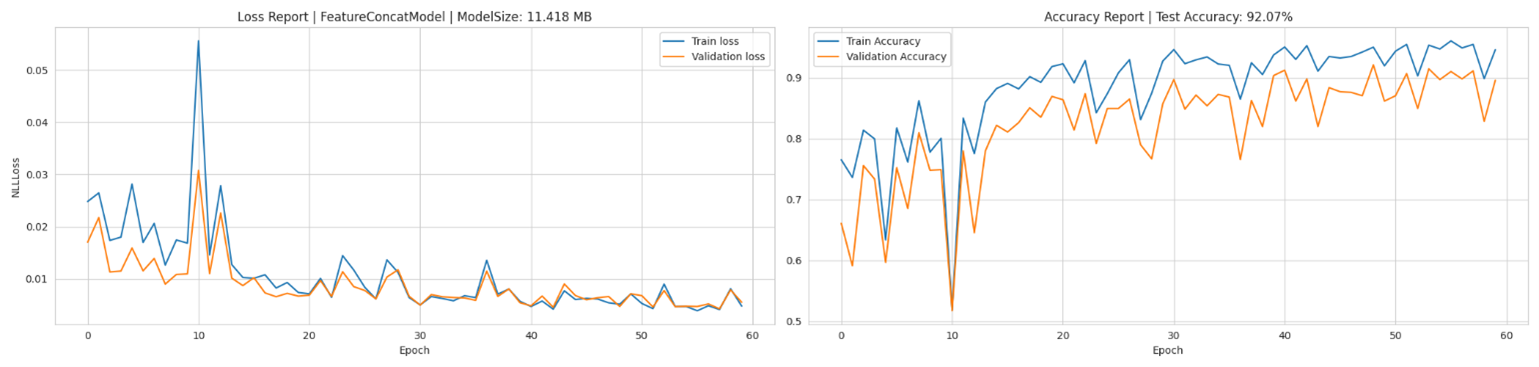
\includegraphics{fig7.png}}
\caption{Training result for feature concatenation approach On model Net 10.}
\label{fig7}
\end{figure*}
Lastly, we explored the graph classification based on PointNet features approach as our fourth network. 
Again, a feature vector of 10 dimensions, comprising XYZ coordinates and centrality metrics, was utilized for 
training. The training outcomes for this graph-based classification approach are illustrated in Fig.~\ref{fig8}''. 
\begin{figure*}[b]
\centering{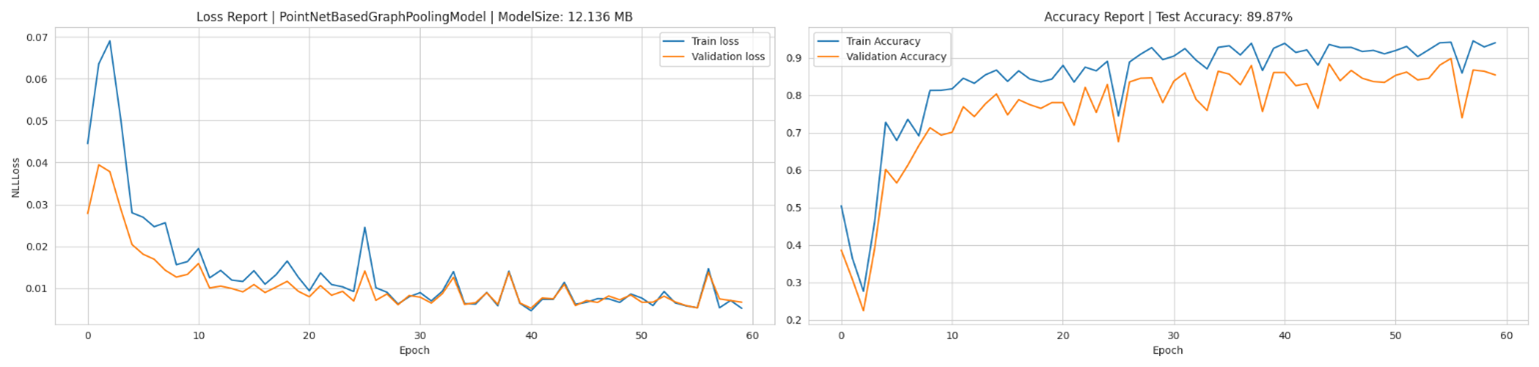
\includegraphics{fig8.png}}
\caption{Training result for graph classification based on PointNet features approach On model Net 10.}
\label{fig8}
\end{figure*}
In all four networks, the same sets were used for training and testing, ensuring a fair and unbiased evaluation
 of their performance. The inclusion of centrality metrics in the feature vectors enhances the models' capability 
 to capture essential node connectivity information, contributing to improved classification accuracy. 
 These comprehensive experiments allow us to gain valuable insights into the efficacy of combining SAGPool and 
 PointNet architectures and highlight their potential to enhance point cloud classification tasks. The results obtained 
 from these experiments play a pivotal role in shaping our understanding of the proposed fusion approaches and their practicality
  in real-world applications. Also the summary of the training results is presented in Table.~\ref{tab}




\begin{table*}[t]
    
\caption{Training Results of Four Networks. This table provides a comprehensive overview of the results obtained from training four networks, including traditional PointNet, hierarchical SAGPool, feature concatenation, and Graph Classification based on PointNet Features approaches. For each network, the features used during training, test accuracy achieved, model size, and corresponding learning rate are reported. The best-performing results are denoted by bold font, while the second-best results are underlined, offering valuable insights into the performance of each approach}
\begin{center}
\begin{tabular}{|c|c|c|c|c|}
\hline
\textbf{Network} & \textbf{\textit{Features}}& \textbf{\textit{Acc}}& \textbf{\textit{Size}}& \textbf{\textit{LR}} \\
\hline
PointNet& 3 (XYZ)&	91.85& 13.259 MB& 0.001 \\
\hline
Hierarchical SAGPool&	3 (XYZ) + 7 (Centralities)& 87.89&	0.3 MB&	0.01 \\
\hline
FeatureConcat&	3 (XYZ) + 7 (Centralities)&	92.07&	11.418 MB&	0.005 \\
\hline
PointNetBasedGraphPooling&	3 (XYZ) + 7 (Centralities)&	89.87&	12.136 MB&	0.005 \\
\hline

\end{tabular}
\label{tab}

\end{center}
\end{table*}

{
    \color{red}
     \# Todo GradCam loss and accuracy plots  (Choupan) \\
     \# Todo convergense Analysis ,all fetures results , modelNEt40 results  [Should be done by Ms Atyabi]
}

\section{CONCLUSION}

\subsection{Networks Comparison}
In terms of model size, the Hierarchical SAGPool network stands out as the most compact, occupying only 0.3 MB. On the other hand, the FeatureConcat approach exhibits a larger model size, consuming 11.418 MB. The PointNetBasedGraphPooling network follows closely, with a model size of 12.136 MB, while PointNet takes up the most space with 13.259 MB.

When considering test accuracy, FeatureConcat outperforms other networks, achieving an impressive accuracy of 92.07%. PointNetBasedGraphPooling closely follows with an accuracy of 89.87%, demonstrating the effectiveness of combining PointNet and SAGPool features. PointNet ranks third with an accuracy of 85.35%, and Hierarchical SAGPool achieves 81.61% accuracy.

Regarding generalization, FeatureConcat showcases the best performance, successfully capturing complex patterns and dependencies in the data. PointNetBasedGraphPooling also exhibits strong generalization capabilities, owing to the fusion of local and global features. PointNet performs well in generalizing to unseen data, while Hierarchical SAGPool shows slightly lower generalization performance.

In conclusion, the FeatureConcat approach strikes a balance between model size and test accuracy, presenting a superior choice for point cloud classification tasks. PointNetBasedGraphPooling follows closely, showcasing promising results by leveraging the intersection of PointNet and SAGPool. The PointNet architecture excels in efficiency and is a viable option for point cloud classification. The hierarchical SAGPool approach offers a compact model size but falls slightly behind in accuracy and generalization. Overall, the fusion approaches demonstrate considerable potential for enhancing point cloud classification, with FeatureConcat standing out as the most robust and effective solution in this study.
\subsection{Conclusion and review the report}
The task of this research was to explore and enhance the point cloud classification using feature engineering, particularly by incorporating graph-based representations and node centralities. To achieve this, two main traditional approaches, PointNet and SAGPool, were employed as the basis for investigation. The study focused on developing and evaluating two new fusion approaches, namely FeatureConcat and PointNetBasedGraphPooling, which combined the strengths of PointNet and SAGPool architectures.

Feature engineering played a crucial role in improving the representation of point cloud data. By building graphs and utilizing node centralities, the relationships and significance of each point in the point cloud were effectively captured. The inclusion of node centralities, such as betweenness, closeness, Katz, PageRank, eigenvector, harmonic, and load centralities, provided valuable connectivity information, aiding in more accurate and robust classification.

The traditional approaches, PointNet and SAGPool, served as fundamental baselines for the new fusion approaches. PointNet, being a pioneering architecture in point cloud classification, showcased efficiency in handling unordered data. SAGPool, on the other hand, demonstrated the capability of adaptive feature pooling using graph structures, proving beneficial in capturing global context.

The newly proposed approaches, FeatureConcat and PointNetBasedGraphPooling, exhibited significant improvements in point cloud classification. FeatureConcat effectively combined high-level features from PointNet and SAGPool, leading to remarkable accuracy gains. PointNetBasedGraphPooling leveraged the intersection of PointNet and SAGPool features, further enhancing classification performance.

The results indicated that the fusion of SAGPool and PointNet significantly improved test accuracy compared to the individual approaches. FeatureConcat achieved an impressive test accuracy of 92.07%, while PointNetBasedGraphPooling closely followed with 89.87%. These findings demonstrated the value of integrating graph-based pooling and centralities with PointNet's feature extraction capabilities, resulting in more informative and robust representations for point cloud classification.

In conclusion, this research successfully explored and enhanced point cloud classification through feature engineering. The incorporation of graph-based representations and node centralities proved instrumental in achieving more accurate and efficient classification. The newly proposed fusion approaches, FeatureConcat and PointNetBasedGraphPooling, demonstrated remarkable performance gains, showcasing their potential in advancing point cloud classification tasks. This study contributes valuable insights and practical approaches for handling complex point cloud data and lays the foundation for further research in this field.

\subsection{Future works}
\begin{itemize}
\item 	Diverse Dataset Exploration: To further validate the robustness and generalization of the proposed fusion approaches, it is essential to explore and evaluate their performance on different datasets with varying complexities and sizes. Investigating datasets that encompass a wider range of 3D objects and scenes will provide deeper insights into the approaches' adaptability and effectiveness in real-world scenarios.

\item 	Extended Training Analysis: In future research, the effect of extended training periods should be explored to understand how longer training durations impact the convergence and overall performance of the fusion approaches. Additionally, investigating the influence of different batch sizes and learning rates on training dynamics and model performance will help in optimizing the training process and achieving higher accuracy.


\item 	Fine-tuning of Fusion Approach Components: The proposed fusion approaches, FeatureConcat and PointNetBasedGraphPooling, utilize MLP and 1D convolution layers, dropout, and batch normalization. Fine-tuning these components and hyperparameters can further enhance the network's performance and efficiency. Optimizing these details will lead to improved feature extraction and pooling, contributing to better classification results.
The source code for the proposed fusion approaches, along with the experimental setup and dataset preparation, is available at the following link: https://github.com/MohsenEbadpour/PointNet-meets-Self-Attention-Graph-Pooling-A-Synergistic-Approach-to-Point-Cloud-Classification. Researchers are encouraged to contribute to the development and completion of this work. Collaborating on refining the fusion approaches, exploring additional datasets, and conducting in-depth experiments will enhance the credibility and significance of the findings.

Furthermore, we extend an invitation to fellow researchers to join efforts in preparing and submitting this research to a reputable academic conference or journal. By collaborating and sharing insights, we can collectively advance the field of point cloud classification and foster meaningful discussions within the scientific community.

\end{itemize}







\section*{References}
{
    \color{red}
    ready in the copy of the report
}

% \begin{thebibliography}{00}
% \bibitem{b1} G. Eason, B. Noble, and I. N. Sneddon, ``On certain integrals of Lipschitz-Hankel type involving products of Bessel functions,'' Phil. Trans. Roy. Soc. London, vol. A247, pp. 529--551, April 1955.
% \bibitem{b2} J. Clerk Maxwell, A Treatise on Electricity and Magnetism, 3rd ed., vol. 2. Oxford: Clarendon, 1892, pp.68--73.
% \bibitem{b3} I. S. Jacobs and C. P. Bean, ``Fine particles, thin films and exchange anisotropy,'' in Magnetism, vol. III, G. T. Rado and H. Suhl, Eds. New York: Academic, 1963, pp. 271--350.
% \bibitem{b4} K. Elissa, ``Title of paper if known,'' unpublished.
% \bibitem{b5} R. Nicole, ``Title of paper with only first word capitalized,'' J. Name Stand. Abbrev., in press.
% \bibitem{b6} Y. Yorozu, M. Hirano, K. Oka, and Y. Tagawa, ``Electron spectroscopy studies on magneto-optical media and plastic substrate interface,'' IEEE Transl. J. Magn. Japan, vol. 2, pp. 740--741, August 1987 [Digests 9th Annual Conf. Magnetics Japan, p. 301, 1982].
% \bibitem{b7} M. Young, The Technical Writer's Handbook. Mill Valley, CA: University Science, 1989.
% \end{thebibliography}
% \vspace{12pt}
% \color{red}
% IEEE conference templates contain guidance text for composing and formatting conference papers. Please ensure that all template text is removed from your conference paper prior to submission to the conference. Failure to remove the template text from your paper may result in your paper not being published.

\end{document}
